\documentclass[11pt,a4paper]{article}

\usepackage[utf8]{inputenc}
\usepackage[T1]{fontenc}
\usepackage{lmodern}
\usepackage[french]{babel}
\usepackage[margin=2.0cm]{geometry}
\usepackage{microtype}
\usepackage{amsmath,amssymb}
\usepackage{booktabs}
\usepackage{array}
\usepackage[table]{xcolor}
\usepackage{graphicx}
\usepackage{caption}
\usepackage{enumitem}
\usepackage[most]{tcolorbox}

\definecolor{navy}{HTML}{1F3864}
\definecolor{bluemid}{HTML}{2E5496}
\definecolor{lightblue}{HTML}{D6E0F0}

\captionsetup{font=small,labelfont={bf,color=navy},labelsep=period}
\graphicspath{{../figures/}}

\newtcolorbox{cle}[1][]{colback=lightblue!40,colframe=navy,boxrule=0.6pt,
  arc=2pt,left=8pt,right=8pt,top=6pt,bottom=6pt,#1}

\title{\vspace{-1.2cm}\color{navy}\bfseries Le test placebo, et la lecture de la carte du courant\\[2pt]
  \large Origine, formule, protocole, résultats, et ce que valent $z$ et $\sigma$
  dans $P=S+zA$}
\author{Kélian Kaddouri}
\date{31 juillet 2026}

\begin{document}
\maketitle
\vspace{-0.9cm}

\begin{cle}
\textbf{Objet.} Cette fiche répond à trois demandes du point du 31/07~: documenter
entièrement le placebo (d'où il vient, sa formule, son protocole), expliquer la carte du
courant de la figure~Z11 et ce que valent les nombres qu'elle affiche, et clarifier
l'interprétation de $z$ et de $\sigma$ dans la décomposition $P=S+zA$. Les trois portent
sur le même objet~: la \textbf{direction} de la contagion, et sur la question de savoir ce
qu'une donnée peut en dire.
\end{cle}

% =====================================================================
\section*{1. Le placebo, en une phrase}

On veut savoir si la direction observée dans les données est un signal ou du bruit. Le
problème est que \textbf{même des données sans aucune direction produisent un déséquilibre},
par simple fluctuation d'échantillonnage, exactement comme cent lancers de pièce ne donnent
jamais cinquante piles exactement. Observer un déséquilibre ne prouve donc rien tant qu'on
ne sait pas ce que le hasard produit tout seul.

Le placebo fournit ce point de comparaison. On fabrique une version des données
\textbf{dont la direction a été détruite volontairement}, tout le reste étant conservé, et
on compare. L'analogie est celle de l'essai clinique~: si le médicament ne fait pas mieux
que la pilule vide, il ne fait rien.

% =====================================================================
\section*{2. D'où il vient}

Le test est introduit dans le script \texttt{2\_donnees/05\_faisabilite\_donnees.py}, sur la
source \textsc{sas} OpRisk Global Data (pertes opérationnelles bâloises, en dollars). Cette
source est la seule des deux étudiées à porter un volume suffisant~: $4329$ transitions
annuelles consécutives sur les catégories de risque de Bâle, soit plusieurs dizaines
d'observations par cellule. C'est précisément parce que le volume ne pose plus problème que
le résultat du placebo est concluant~: l'échec ne peut pas être imputé à la taille de
l'échantillon.

La proposition~3 du script \texttt{6\_contagion\slash 32\_proprietes\_formelles.py} le
reprend pour en tirer la conséquence formelle~: $W$ et $W^{\top}$ partagent la même partie
symétrique et ne diffèrent que par le signe de $A$, elles sont donc également compatibles
avec la donnée. Le script \texttt{6\_contagion\slash 53\_postmortem\_direction.py} applique
\emph{le même} test au corpus de rapports post-incident. Même statistique, deux sources,
deux verdicts opposés~: c'est l'architecture du chapitre~9.

\begin{cle}[colback=orange!8,colframe=orange!70!black]
\textbf{Pourquoi pas le test intuitif du \og temps inversé\fg.} La première idée qui vient
est de comparer la matrice des transitions à celle obtenue en renversant la chronologie.
Elle est \textbf{dégénérée sur un comptage brut}~: renverser la chronologie donne
$M_{\text{inv}}=M^{\top}$ \emph{par construction}, donc une corrélation des asymétries de
$-1$ quel que soit le contenu des données. Ce test ne peut rien prouver. Seul le placebo par
permutation est valide sur des comptages, et il faut le dire explicitement.
\end{cle}

% =====================================================================
\section*{3. La formule}

\textbf{La statistique.} Soit $M$ la matrice des transitions comptées, $M_{jk}$ étant le
nombre de fois où le pilier $k$ est observé après le pilier $j$. On mesure son asymétrie en
norme $L^1$~:
\begin{equation}
  \mathcal{A}(M)\;=\;\frac{\bigl\|M-M^{\top}\bigr\|_1}{2}
  \;=\;\frac12\sum_{j,k}\bigl|M_{jk}-M_{kj}\bigr| .
  \label{eq:asym}
\end{equation}
Lecture directe~: $\mathcal{A}$ compte le \textbf{surplus de transitions} d'un sens sur
l'autre, sommé sur toutes les paires. Si la matrice est parfaitement symétrique,
$\mathcal{A}=0$. Plus elle penche, plus $\mathcal{A}$ est grand. C'est un décompte, pas un
score normalisé, et son unité est le nombre de transitions.

\textbf{La loi nulle.} Sous $H_0$ \og il n'existe aucune direction privilégiée\fg, on
construit une distribution de référence en \textbf{permutant les années à l'intérieur de
chaque entité}. L'ensemble des catégories touchées chaque année est conservé intact, la
structure d'adjacence entre années consécutives aussi, et seul l'\textbf{ordre} est détruit.
On recompte $M$ sur ces données permutées et on recalcule $\mathcal{A}$, opération répétée
$30$ fois. Formellement, avec $\mathcal{A}^{(r)}$ la valeur au tirage~$r$~:
\begin{equation}
  z\;=\;\frac{\mathcal{A}(M_{\text{obs}})-\overline{\mathcal{A}^{\,\text{null}}}}
       {\widehat{s}\bigl(\mathcal{A}^{\,\text{null}}\bigr)} .
  \label{eq:z}
\end{equation}

\begin{cle}
\textbf{Ce qui fait la validité du test.} La permutation \textbf{conserve tout sauf la
direction}~: mêmes entités, mêmes fréquences marginales, mêmes co-occurrences, même volume,
même structure de déclaration. La seule différence entre le groupe réel et le groupe témoin
est l'antériorité. Un écart nul ne peut donc pas être imputé à une particularité des
données~; il ne peut être imputé qu'à l'absence de direction dans ces données.
\end{cle}

% =====================================================================
\section*{4. Les résultats}

\begin{center}
\small
\begin{tabular}{@{}l r r r l@{}}
\toprule
\textbf{Source} & \textbf{$\mathcal{A}$ observée} & \textbf{$\mathcal{A}$ sous placebo} &
\textbf{$z$} & \textbf{Verdict} \\
\midrule
OpRisk, pas annuel & $119$ & $128 \pm 27$ & $-0{,}33$ & aucun signal directionnel \\
7 rapports post-incident & \multicolumn{2}{c}{\emph{(même protocole, par arête)}} &
$+3{,}93$ & signal net, $p=0{,}0004$ \\
\bottomrule
\end{tabular}
\end{center}

\medskip
Sur OpRisk, l'asymétrie observée est \textbf{sous} la moyenne du bruit. Ce n'est pas
\og un peu trop faible pour conclure\fg, c'est en dessous de ce que produit le hasard.
Un test binomial par paire, sous $H_0: p=0{,}5$, le confirme~: aucune paire ne survit à la
correction de Bonferroni. Le pas annuel a lessivé la direction.

Sur le corpus de post-mortems, le même test est franchi largement. \textbf{On change de
type de donnée, pas de méthode}, et le signal apparaît. C'est ce qui prouve que le problème
venait de la donnée et non de la statistique.

% =====================================================================
\section*{5. Ce que le placebo représente vraiment}

Trois lectures, de la plus faible à la plus forte.

\textbf{(i) Lecture empirique.} Les données annuelles agrégées ne portent pas
d'information directionnelle exploitable.

\textbf{(ii) Lecture en termes d'irréversibilité.} Le placebo est un test de
$\sigma=0$, où $\sigma$ est la production d'entropie définie en section~7. Autrement dit,
\textbf{la co-occurrence observée est compatible avec une dynamique réversible}. C'est un
énoncé plus précis que \og je n'ai pas trouvé de direction\fg.

\textbf{(iii) Lecture théorique, la plus forte.} Le test \textbf{ne pouvait pas} passer. La
statistique $\mathcal{A}$ de l'équation~\eqref{eq:asym} est construite sur des transitions
comptées sans ordre~; toute statistique de ce type prend la même valeur sur un processus et
sur son renversé, et ne peut donc pas identifier un courant qui, lui, change de signe sous
ce renversement. Aucun volume de données annuelles ne le réparera. La démonstration est
dans la fiche \emph{socle mathématique de $W=S+A$}.

% =====================================================================
\section*{6. La carte du courant, et ce que valent les nombres affichés}

\begin{center}
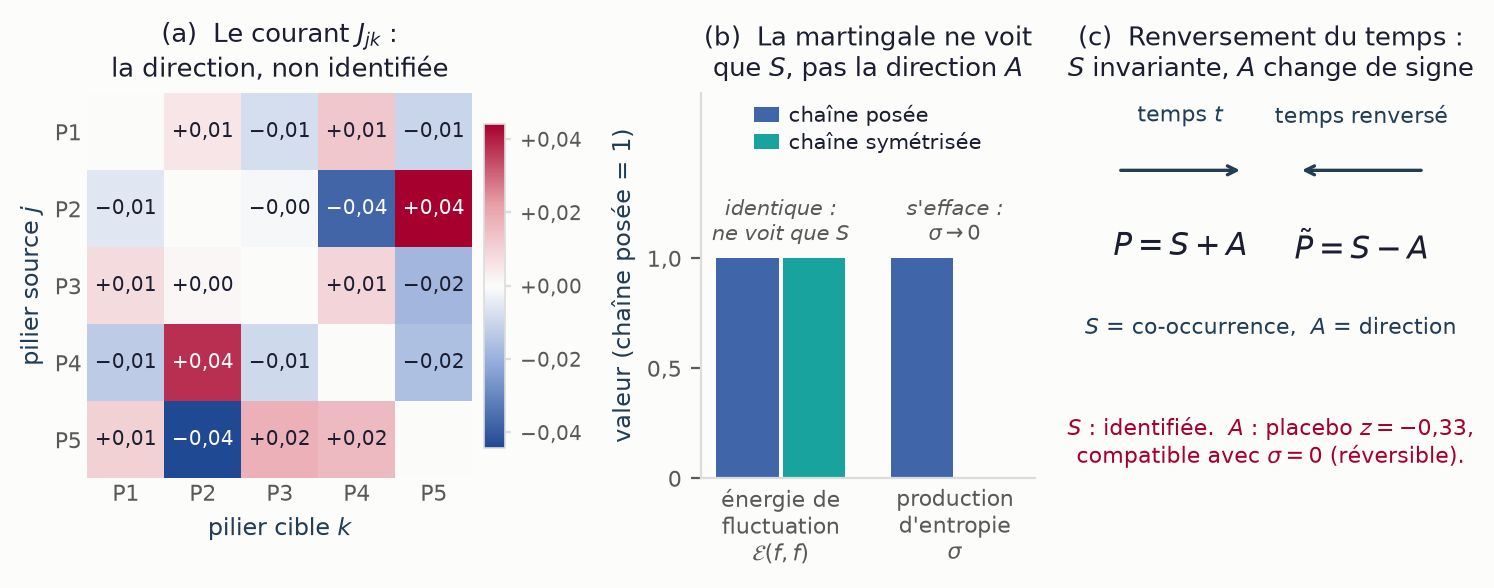
\includegraphics[width=\linewidth]{Z11_reversibilite_martingale.png}
\captionof{figure}{Les trois panneaux de la figure~Z11 (script~40).}
\end{center}

\subsection*{Panneau (a)~: la carte du courant}

Ce n'est \textbf{pas} une carte de corrélation, et c'est le point à ne pas confondre. Une
corrélation est symétrique et n'a pas de sens de lecture. Ici, chaque case porte le
\textbf{courant net de probabilité}
\begin{equation}
  J_{jk}\;=\;\pi_j P_{jk}-\pi_k P_{kj},
  \label{eq:courant}
\end{equation}
qui est \emph{antisymétrique}~: $J_{jk}=-J_{kj}$, la carte est donc rouge d'un côté de la
diagonale et bleue de l'autre, par construction.

\textbf{L'unité.} $\pi_j P_{jk}$ est la probabilité, en régime stationnaire, d'observer la
transition $j\to k$ sur un pas. $J_{jk}$ est donc une \textbf{différence de probabilités},
sans dimension, comprise entre $-1$ et $1$. L'échelle de couleur est centrée sur zéro et
bornée par $\max|J|=0{,}0443$.

\textbf{Ce que vaut un $+0{,}04$.} Prenons la case la plus forte, $J_{25}=+0{,}0443$. Elle
se décompose ainsi~:
\[
  \underbrace{\pi_2 P_{25}}_{0{,}263\times0{,}400\;=\;0{,}105}
  \;-\;
  \underbrace{\pi_5 P_{52}}_{0{,}214\times0{,}286\;=\;0{,}061}
  \;=\;0{,}044 .
\]
Traduction en clair~: sur mille transitions observées à long terme, environ \textbf{105
vont de P2 vers P5} et \textbf{61 vont de P5 vers P2}. Il reste un \textbf{surplus net de
44 transitions pour mille} dans le sens P2 vers P5. C'est cela, le $+0{,}04$.

\medskip
\begin{center}
\small
\begin{tabular}{@{}l r l@{}}
\toprule
\textbf{Paire} & \textbf{$|J|$} & \textbf{Lecture} \\
\midrule
P2 $\to$ P5 & $0{,}0443$ & $44$ transitions nettes pour mille, le courant dominant \\
P4 $\to$ P2 & $0{,}0377$ & $38$ pour mille, les tiers alimentent les incidents \\
P5 $\to$ P3 & $0{,}0181$ & $18$ pour mille \\
\bottomrule
\end{tabular}
\end{center}

\medskip
\textbf{Un ordre de grandeur à assumer.} Ces valeurs sont \emph{petites} en valeur absolue,
et c'est normal~: elles sont des différences de probabilités par pas, donc bornées par la
probabilité elle-même. Ce qui compte est leur \textbf{rapport} à ces probabilités~: pour la
paire P2/P5, le surplus représente $44/(105+61)\approx 27\,\%$ du trafic total de la paire.
Le courant n'est pas marginal, l'échelle de l'axe seule le laisse croire.

\textbf{Attention à $\pi$.} La loi stationnaire vaut ici $\pi=(0{,}131;\,0{,}263;\,0{,}200;
\,0{,}192;\,0{,}214)$ pour P1 à P5. C'est un profil de \textbf{réceptacle}, l'endroit où la
marche s'accumule, à ne pas confondre avec l'ordre des \textbf{sources}. P2 a le $\pi$ le
plus élevé parce qu'il reçoit, pas parce qu'il déclenche.

\subsection*{Panneau (b)~: pourquoi deux barres à la même hauteur}

Les valeurs sont \textbf{normalisées à la chaîne posée}, qui vaut donc $1$ dans les deux
groupes. Ce panneau ne montre pas des niveaux, il montre \textbf{ce qui change et ce qui ne
change pas} quand on symétrise la chaîne, c'est-à-dire quand on efface la direction.

À gauche, l'énergie de fluctuation (la forme de Dirichlet, soit la variation quadratique de
la martingale) est \textbf{identique} avant et après symétrisation. Vérifié sur $2000$
fonctions test tirées au hasard, écart maximal $1{,}8\times10^{-15}$, c'est-à-dire zéro
numérique. La fluctuation ne voit pas la direction.

À droite, la production d'entropie passe de $0{,}0700$ à $5{,}4\times10^{-33}$, donc
s'efface entièrement. Toute l'irréversibilité était dans la partie antisymétrique.

\textbf{C'est le c\oe{}ur de la figure}~: une même opération laisse une quantité intacte et en
annule une autre. Ce qu'une donnée de co-occurrence mesure, c'est la première.

\subsection*{Panneau (c)~: le schéma}

Il énonce l'identité~: la chaîne renversée dans le temps a pour flux $S-A$. La partie
symétrique est invariante, la partie antisymétrique change de signe. Les écarts numériques
mesurés sont de l'ordre de $10^{-17}$, donc l'identité est exacte.

% =====================================================================
\section*{7. $z$ et $\sigma$ dans $P=S+zA$}

L'écriture $P=S+zA$ introduit un \textbf{paramètre d'amplitude} $z$ sur la partie
directionnelle. Elle est utile parce qu'elle sépare deux questions que la notation
$P=S+A$ confond.

\begin{center}
\small
\begin{tabular}{@{}l p{5.2cm} p{6.6cm}@{}}
\toprule
& \textbf{$z$} & \textbf{$\sigma$} \\
\midrule
Nature & paramètre, réglable & fonctionnelle, calculée à partir de la chaîne \\
Domaine & $[-1,1]$ & $[0,+\infty[$ \\
Signe & porte le \textbf{sens} & toujours positif, ne porte \textbf{aucun} sens \\
$z=0$ & chaîne réversible & $\sigma=0$ \\
$z=1$ & la chaîne posée & $\sigma=0{,}0700$ \\
$z=-1$ & toutes les flèches retournées & $\sigma=0{,}0700$, \emph{la même} \\
Ce qu'il mesure & \emph{dans quel sens} et \emph{à quelle force} & \emph{à quel point} le
processus est irréversible \\
\bottomrule
\end{tabular}
\end{center}

\subsection*{7.1. Deux lectures de $z$, à ne pas confondre}

L'écriture $P=S+zA$ est ambiguë tant qu'on n'a pas dit si $z$ est \emph{un} nombre ou
\emph{dix}. Les deux lectures existent et ne disent pas la même chose.

\textbf{Lecture globale, $z$ scalaire.} On fixe un motif de direction $A$ une fois pour
toutes, celui du classeur d'expert par exemple, et $z\in[-1,1]$ n'en règle que
l'\textbf{intensité}~: $z=1$ donne la chaîne posée, $z=0$ la chaîne réversible, $z=-1$
toutes les flèches retournées. C'est \textbf{un seul degré de liberté}. Cette lecture ne
peut pas changer \emph{quel} pilier précède \emph{quel} autre, elle ne fait que renforcer ou
affaiblir un ordre déjà choisi. Elle est utile pour un graphique de sensibilité, elle est
insuffisante pour représenter l'ignorance.

\textbf{Lecture par paire, $z_{jk}$ vectoriel.} C'est celle du mémoire. Chaque paire porte
son propre curseur~:
\begin{equation}
  A_{jk}\;=\;z_{jk}\,t\,S_{jk},
  \qquad z_{jk}\in[-1,1],
  \qquad j<k,
  \label{eq:zpaire}
\end{equation}
soit \textbf{dix degrés de liberté}, un par paire de piliers. Le paramètre $t\in[0,1]$ est
l'amplitude maximale d'asymétrie autorisée, commune à toutes les paires, et les $z_{jk}$
portent chacun un sens indépendant. Les \textbf{$2^{10}=1024$ sommets} du mémoire sont
exactement les configurations $z_{jk}=\pm1$, c'est-à-dire tous les choix de sens possibles à
amplitude maximale.

\textbf{La contrainte de faisabilité.} Un flux doit rester positif, donc $S_{jk}\pm
A_{jk}\ge0$, ce qui impose $|A_{jk}|\le S_{jk}$ et justifie la borne $t\le1$. À $t=1$, les
$1024$ sommets décrivent l'\textbf{ignorance totale} sur la direction~: c'est le régime dans
lequel le capital est borné dans $[6858;8697]$.

\subsection*{7.2. Ce que $\sigma$ voit, et ce qu'elle ne voit pas}

En regroupant les termes par paire non ordonnée, la production d'entropie s'écrit comme une
\textbf{somme de dix contributions indépendantes}~:
\begin{equation}
  \sigma\;=\;\sum_{j<k}\,2A_{jk}\,
  \ln\!\frac{S_{jk}+A_{jk}}{S_{jk}-A_{jk}} .
  \label{eq:sigma-paires}
\end{equation}

\textbf{Proposition.} \emph{Chaque terme de~\eqref{eq:sigma-paires} est une fonction paire de
$A_{jk}$~: remplacer $A_{jk}$ par $-A_{jk}$ change le signe des deux facteurs et laisse le
produit inchangé. Donc $\sigma$ ne dépend que des amplitudes $|A_{jk}|$, et pas d'un seul des
dix signes.}

\begin{cle}[colback=orange!8,colframe=orange!70!black]
\textbf{Le résultat exact, et c'est la clarification demandée.} \textbf{Les $1024$ sommets
de l'ensemble admissible ont tous rigoureusement la même production d'entropie.} Vérifié
numériquement~: amplitude entre le minimum et le maximum sur les $1024$ configurations,
$0{,}0\times10^{0}$, pas une erreur d'arrondi, un zéro exact.

Et pourtant ces mêmes $1024$ sommets étalent le capital de $6858$ à $8697$~M, soit
$27\,\%$ d'écart. \textbf{Un scalaire constant sur tout l'ensemble, et un capital qui y
varie d'un quart~:} c'est l'énoncé le plus net du problème d'identification du mémoire.
$\sigma$ mesure \emph{combien} de direction il y a, jamais \emph{laquelle}.
\end{cle}

\medskip
\textbf{Conséquence sur le programme de recherche.} Même une méthode qui estimerait
parfaitement $\sigma$ sur des données ne réduirait pas la bande de capital d'un seul euro,
puisqu'elle donnerait une quantité identique en tout point de l'ensemble. Ce n'est donc pas
$\sigma$ qu'il faut chercher à mesurer, mais les \textbf{signes} $z_{jk}$, un par un. C'est
exactement ce que fait le corpus de post-mortems, et c'est pourquoi la valeur d'information
se hiérarchise \emph{par paire} et non globalement.

\medskip
\textbf{Le comportement près de la réversibilité.} En développant
$\ln\frac{1+x}{1-x}\approx 2x$ avec $x=A_{jk}/S_{jk}$~:
\begin{equation}
  \sigma\;\approx\;4\sum_{j<k}\frac{A_{jk}^2}{S_{jk}}
  \qquad (A\to0),
  \label{eq:sigma-quad}
\end{equation}
soit $\sigma(z)\approx 4z^2\sum_{j<k}A_{jk}^2/S_{jk}$ dans la lecture globale. Vérification
numérique du rapport exact sur approché~: $2{,}022$ à $z=0{,}30$, puis $2{,}0024$,
$2{,}0002$ et $2{,}0000$ à $z=0{,}10$, $0{,}03$ et $0{,}01$. L'approximation est correcte,
et la convergence en $z^2$ est nette.

$\sigma$ est donc \textbf{plate} au voisinage de la réversibilité~: une direction faible ne
produit qu'une irréversibilité du second ordre. C'est une raison supplémentaire, et
indépendante du volume de données, pour laquelle une direction faible est très difficile à
détecter. La quantité qu'on cherche s'annule au premier ordre.

% =====================================================================
\section*{8. Ce que le placebo ne dit pas}

Trois réserves, à porter avec le résultat.

\textbf{Il teste la cohérence, pas l'exogénéité.} Sur le corpus de post-mortems, le
$z=+3{,}93$ établit que le codage est cohérent et non aléatoire. Il n'établit \emph{pas}
que la structure trouvée reflète le terrain plutôt que la convention d'écriture des
rapports d'enquête. Ce confondant, celui de la narration, ne se lève pas par le calcul~:
il appelle une fiabilité inter-juges et une relecture de praticiens.

\textbf{Un test non rejeté n'est pas une preuve d'absence.} Le $z=-0{,}33$ dit que la
donnée est \emph{compatible} avec l'absence de direction, pas que la direction n'existe
pas. Ce qui donne sa force à la conclusion, ce n'est pas le test seul, c'est le test
\emph{plus} le résultat théorique de la section~5(iii).

\textbf{Le nombre de répétitions est modeste.} La loi nulle est estimée sur $30$
permutations pour OpRisk. C'est suffisant pour un $z$ aussi proche de zéro, mais un lecteur
exigeant demandera davantage de tirages pour un résultat limite. Il n'y en a pas ici.

\smallskip
\sloppy
\noindent\footnotesize\textcolor{navy}{\textbf{Sources.}} Placebo~:
\texttt{2\_donnees/05\_faisabilite\_donnees.py} (origine, source OpRisk),
\texttt{6\_contagion/32\_proprietes\_formelles.py} (proposition~3),
\texttt{6\_contagion/53\_postmortem\_direction.py} (application au corpus). Courant et
figure~Z11~: \texttt{6\_contagion/40\_reversibilite\_martingale.py}. Démonstrations~: fiche
\emph{socle mathématique de $W=S+A$}, chapitre~9 du mémoire.

\end{document}
